\documentclass[a4paper,11pt]{article}
\usepackage{amsmath,amsthm,amsfonts,amssymb,amscd,amstext,vmargin,graphics,graphicx,tabularx,multicol} 
\usepackage[francais]{babel}
\usepackage[utf8]{inputenc}  
\usepackage[T1]{fontenc} 
\usepackage{pstricks-add,tikz,tkz-tab,variations}
\usepackage[autolanguage,np]{numprint} 
\usepackage{calc}

\setmarginsrb{1.5cm}{0.5cm}{1cm}{0.5cm}{0cm}{0cm}{0cm}{0cm} %Gauche, haut, droite, haut
\newcounter{numexo}
\newcommand{\exo}[1]{\stepcounter{numexo}\noindent{\bf Exercice~\thenumexo} : }
\reversemarginpar

\newcommand{\bmul}[1]{\begin{multicols}{#1}}
\newcommand{\emul}{\end{multicols}}

\newcounter{enumtabi}
\newcounter{enumtaba}
\newcommand{\q}{\stepcounter{enumtabi} \theenumtabi)  }
\newcommand{\qa}{\stepcounter{enumtaba} (\alph{enumtaba}) }
\newcommand{\initq}{\setcounter{enumtabi}{0}}
\newcommand{\initqa}{\setcounter{enumtaba}{0}}

\newcommand{\be}{\begin{enumerate}}
\newcommand{\ee}{\end{enumerate}}
\newcommand{\bi}{\begin{itemize}}
\newcommand{\ei}{\end{itemize}}
\newcommand{\bp}{\begin{pspicture*}}
\newcommand{\ep}{\end{pspicture*}}
\newcommand{\bt}{\begin{tabular}}
\newcommand{\et}{\end{tabular}}
\renewcommand{\tabularxcolumn}[1]{>{\centering}m{#1}} %(colonne m{} centrée, au lieu de p par défault) 
\newcommand{\tnl}{\tabularnewline}

\newcommand{\trait}{\noindent \rule{\linewidth}{0.2mm}}
\newcommand{\hs}[1]{\hspace{#1}}
\newcommand{\vs}[1]{\vspace{#1}}

\newcommand{\N}{\mathbb{N}}
\newcommand{\Z}{\mathbb{Z}}
\newcommand{\R}{\mathbb{R}}
\newcommand{\C}{\mathbb{C}}
\newcommand{\Dcal}{\mathcal{D}}
\newcommand{\Ccal}{\mathcal{C}}
\newcommand{\mc}{\mathcal}

\newcommand{\vect}[1]{\overrightarrow{#1}}
\newcommand{\ds}{\displaystyle}
\newcommand{\eq}{\quad \Leftrightarrow \quad}
\newcommand{\vecti}{\vec{\imath}}
\newcommand{\vectj}{\vec{\jmath}}
\newcommand{\Oij}{(O;\vec{\imath}, \vec{\jmath})}
\newcommand{\OIJ}{(O;I,J)}


\newcommand{\reponse}[1][1]{%
\multido{}{#1}{\makebox[\linewidth]{\rule[0pt]{0pt}{20pt}\dotfill}
}}

\newcommand{\titre}[5] 
% #1: titre #2: haut gauche #3: bas gauche #4: haut droite #5: bas droite
{
\noindent #2 \hfill #4 \\
#3 \hfill #5

\vspace{-1.6cm}

\begin{center}\rule{6cm}{0.5mm}\end{center}
\vspace{0.2cm}
\begin{center}{\large{\textbf{#1}}}\end{center}
\begin{center}\rule{6cm}{0.5mm}\end{center}
}



\begin{document}
\pagestyle{empty}
\titre{Trouver les bonnes informations pour résoudre un problème}{}{}{6ème}{}


\vspace*{1cm}

{\large \textbf{\underline{PARTIE A :} Garder les informations utiles}}\\


\q Surligner au surligneur toutes les informations utiles pour pouvoir répondre à la question demandée.\\

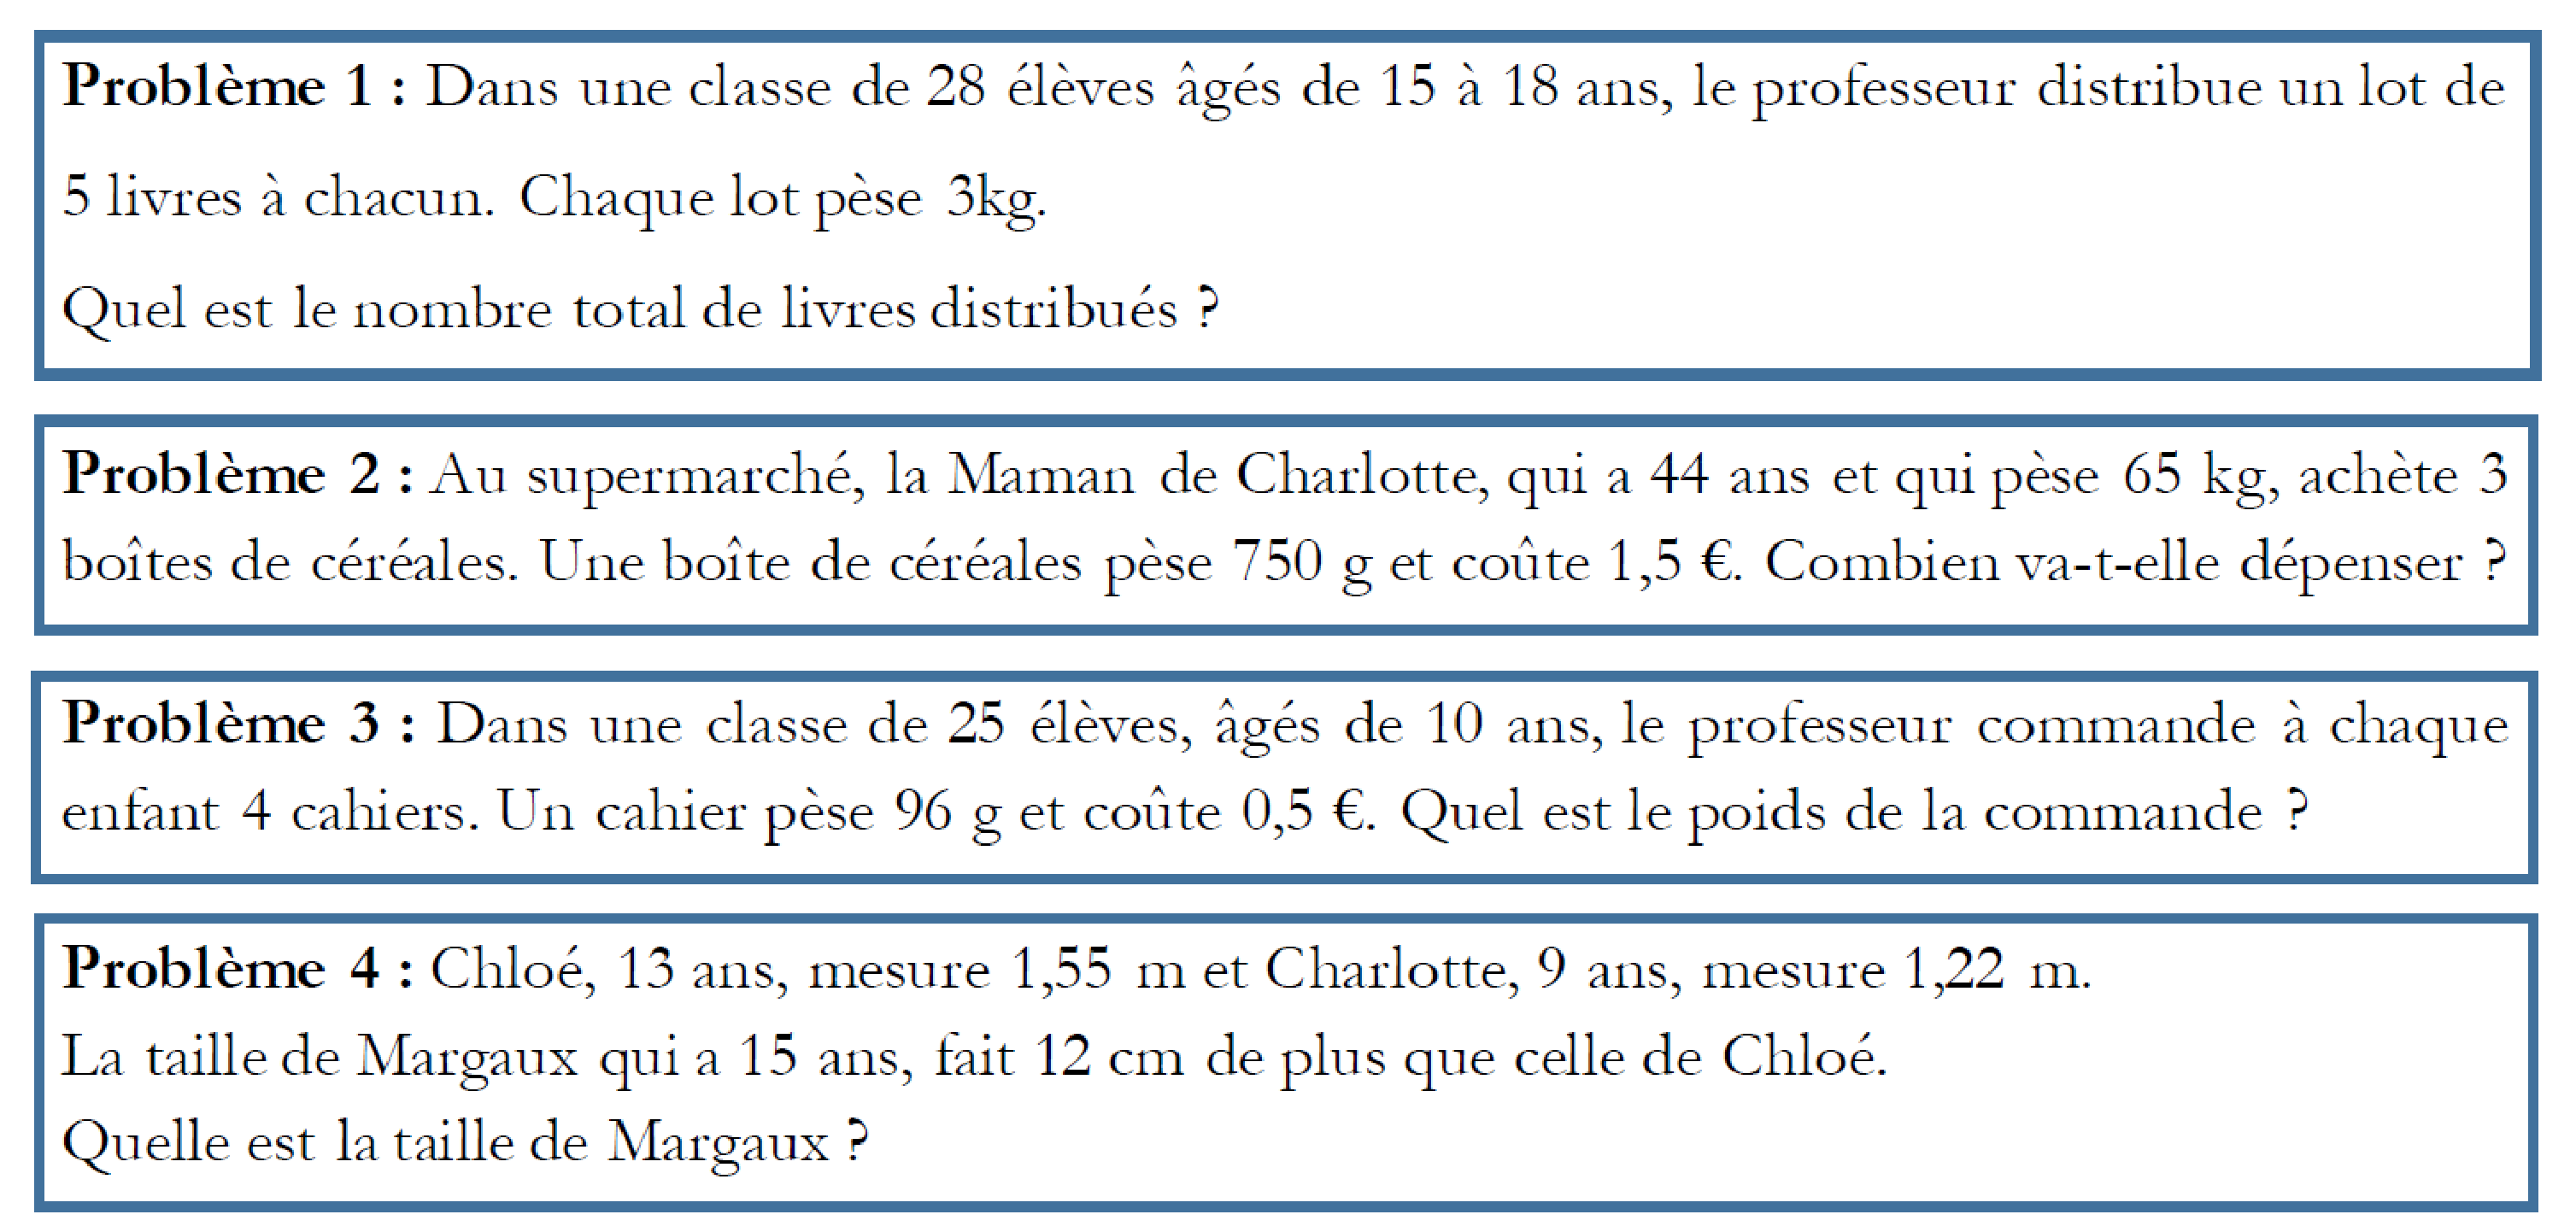
\includegraphics[scale=0.35]{enoncepb1.eps} \\

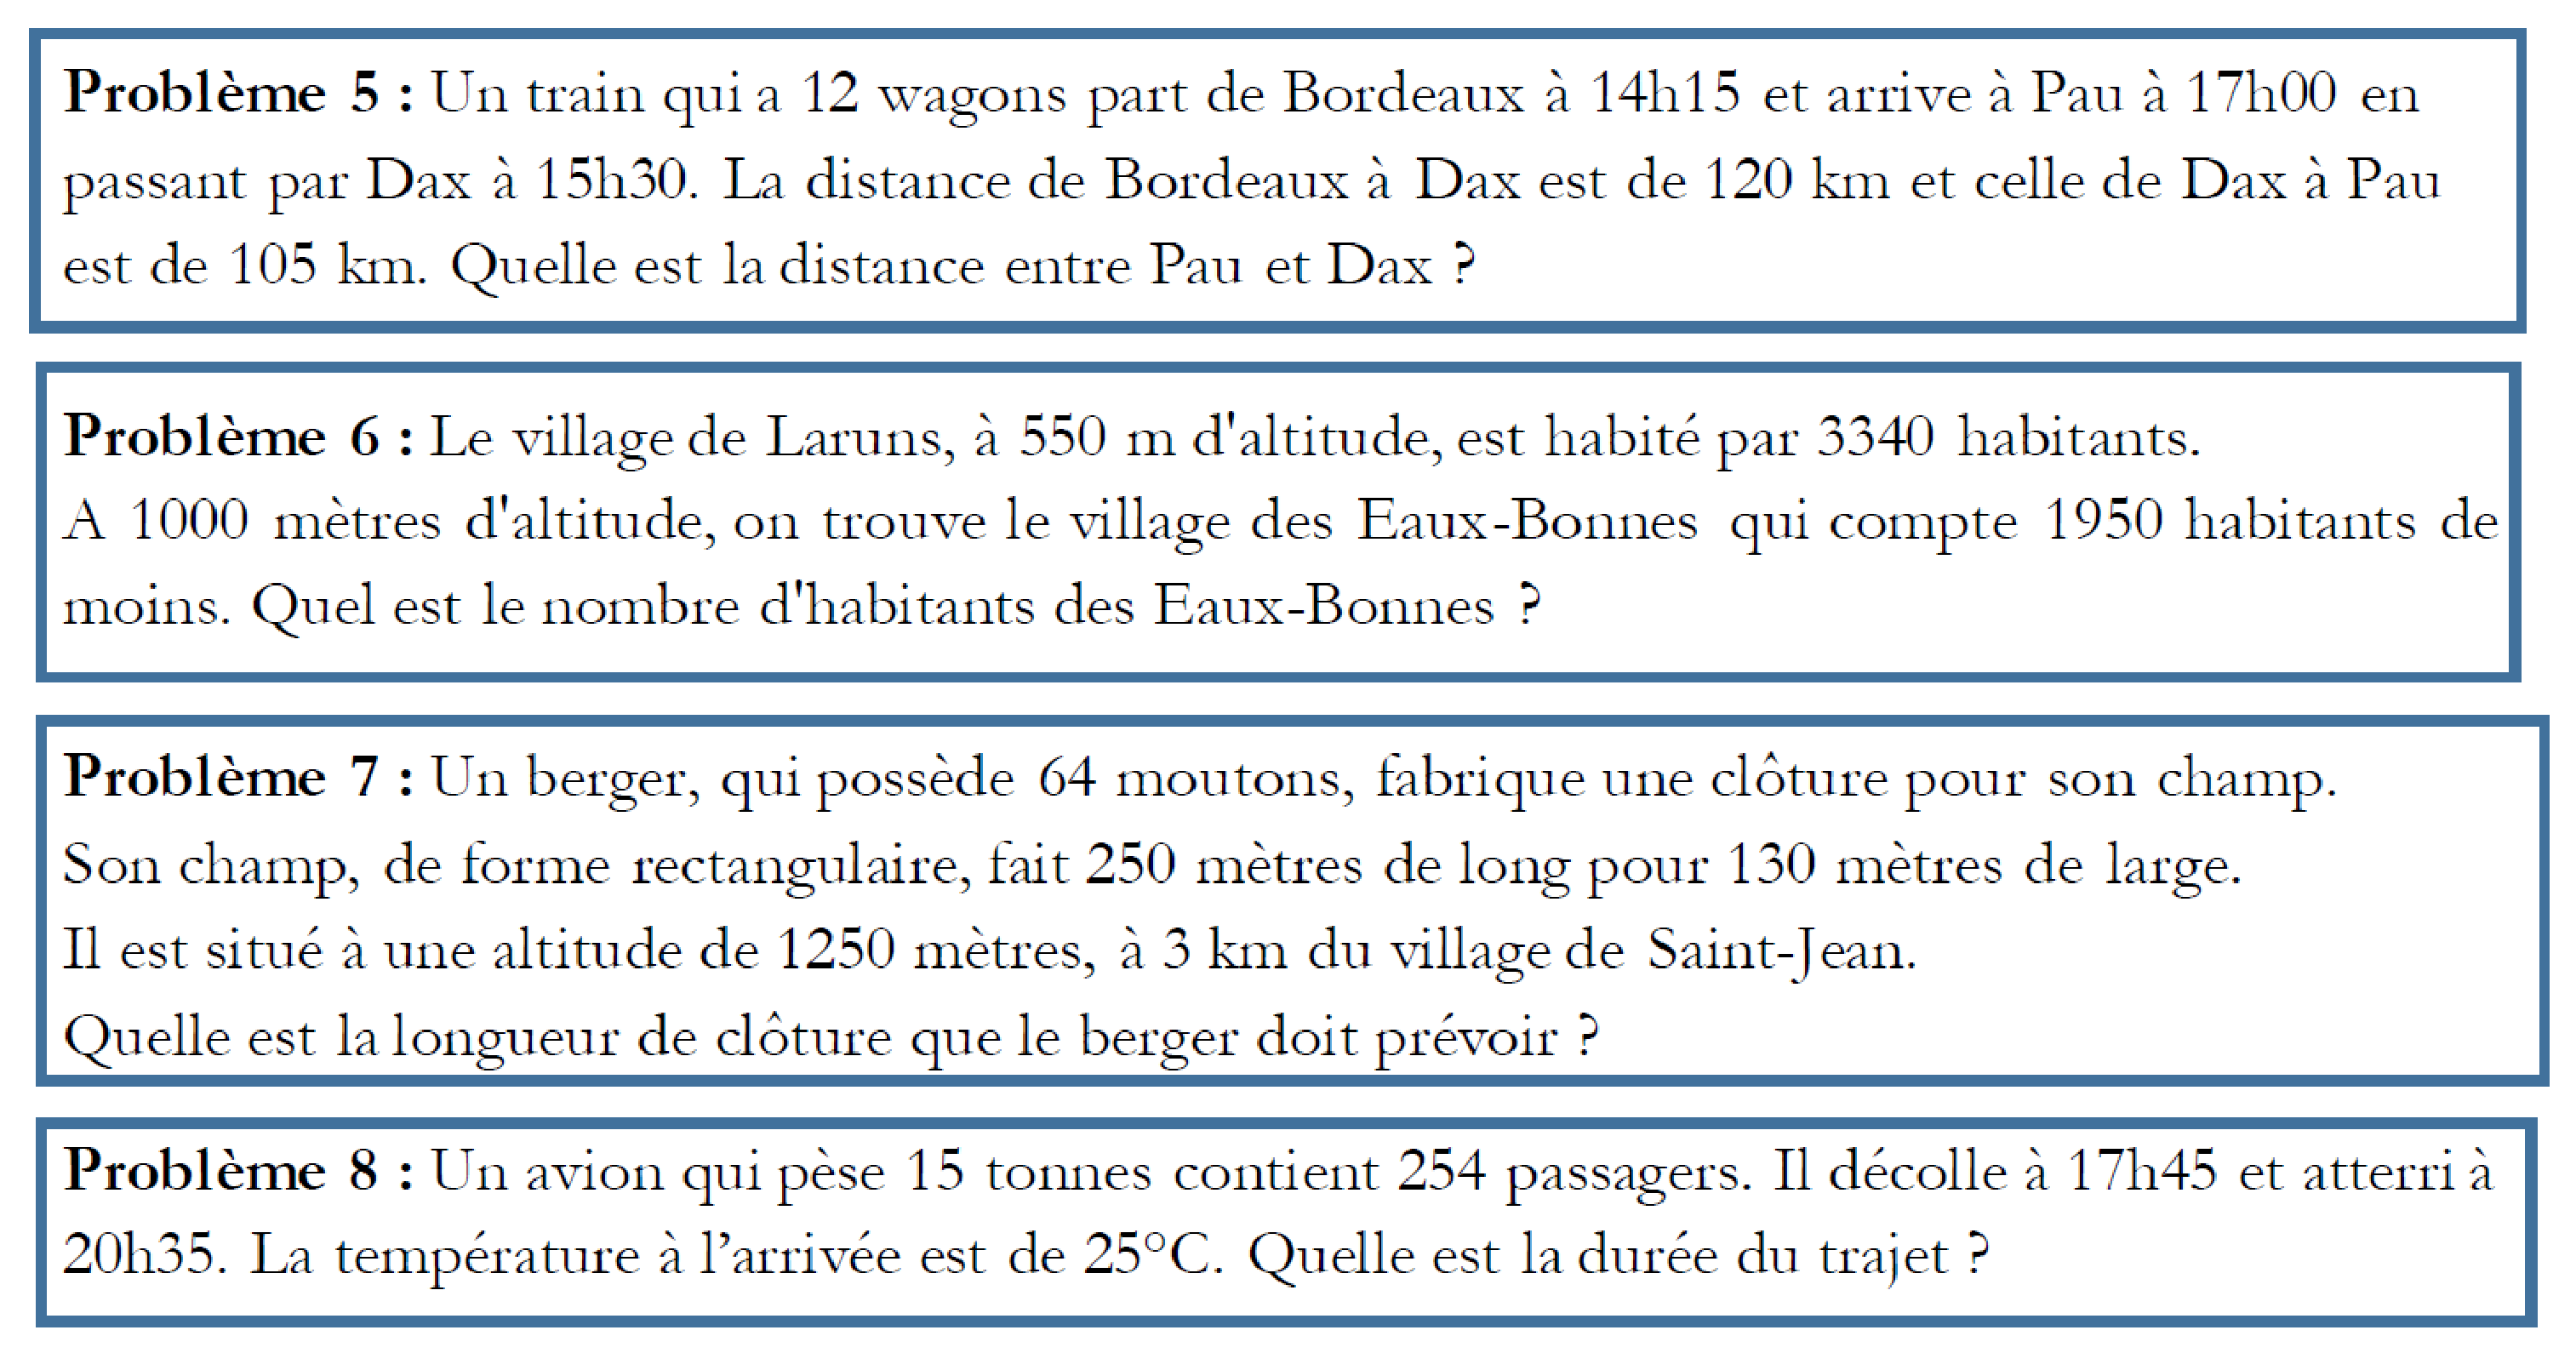
\includegraphics[scale=0.35]{enoncepb2.eps} \\

\q Écrire les calculs qu'ils faut effectuer pour répondre à chaque problème, sans en donner la réponse :\\

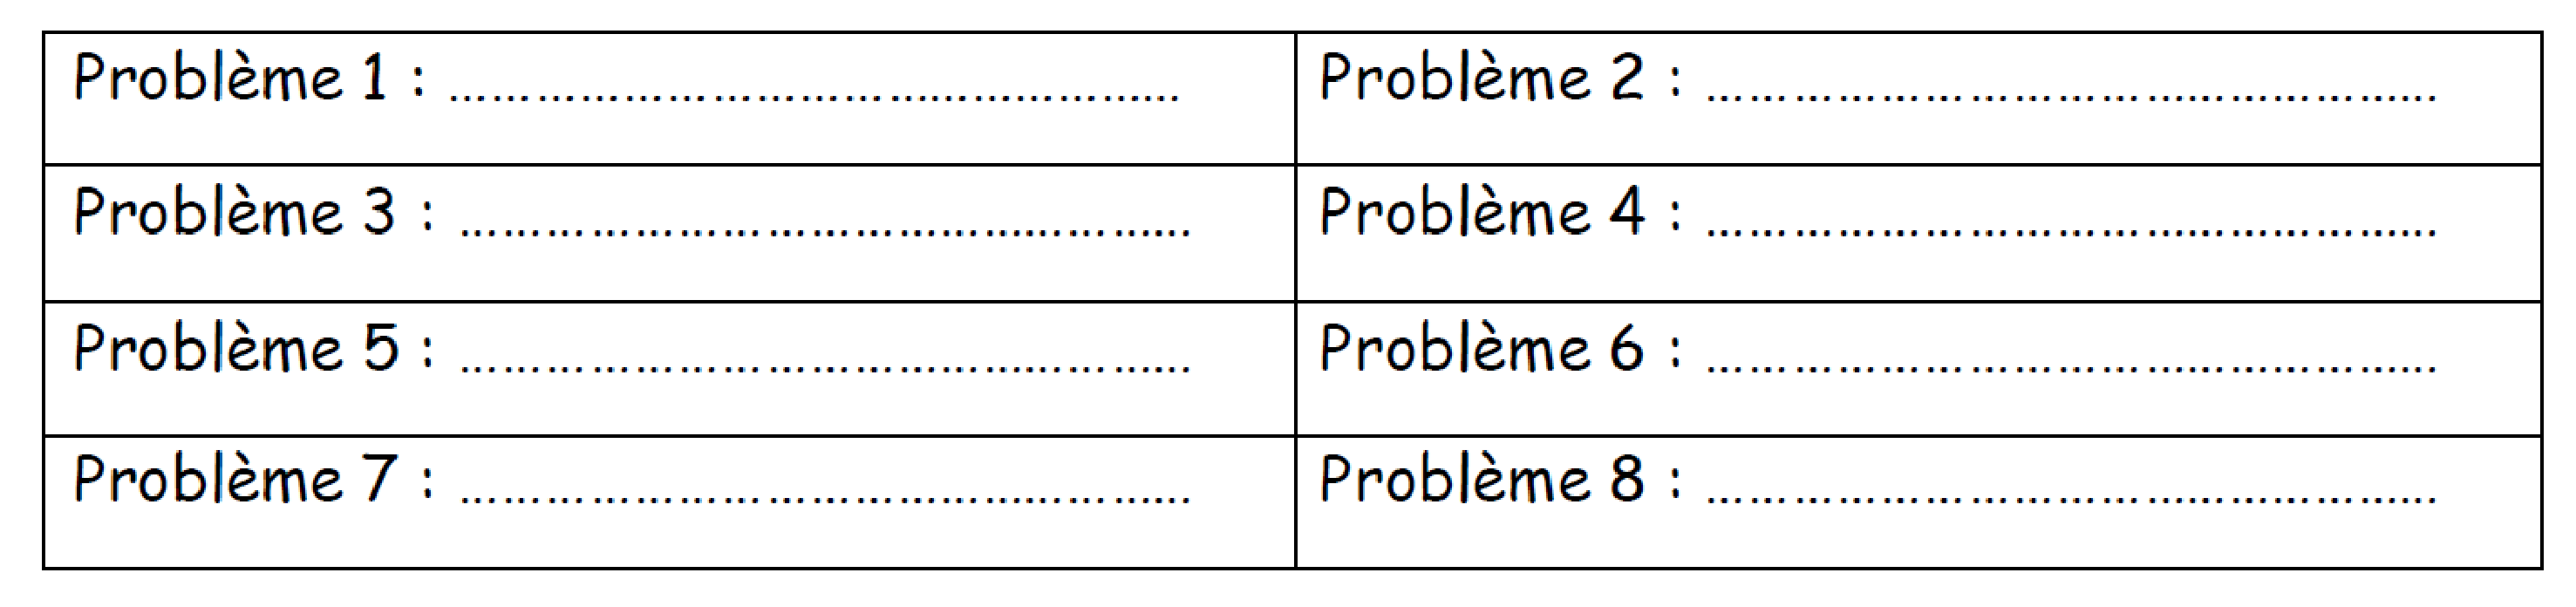
\includegraphics[scale=0.3]{reponsepb.eps} 

\newpage


{\large \textbf{\underline{PARTIE B :} Résoudre un problème}}\\

Sur votre cahier d'exercices, répondez aux problèmes suivants en détaillant bien \textbf{vos calculs} et en finissant par écrire \textbf{une phrase réponse}.\\

\underline{\textbf{PROBLÈME 1 : }}\\

Le métro 13 est parti de Malakoff avec 1 400 personnes. 119 personnes sont montées à l’arrêt de Pernety.\\
Combien de personnes compte le train en arrivant à l'arrêt suivant ?\\

\underline{\textbf{PROBLÈME 2 :} }\\


Paul a ajouté 20 euros dans sa tirelire, grâce au cadeau de sa grand-mère. Il vide alors la tirelire et compte qu'il possède au total 174,50 euros. \\
Combien d'argent y avait-il dans sa tirelire avant le cadeau de sa grand-mère ?\\


\underline{\textbf{PROBLÈME 3 :} }\\

Amina a quitté la maison à 10 h 15 min pour aller faire ses courses ; elle est rentrée à
11 h 05 min.\\
 Combien de
temps est-elle partie ? \\



\underline{\textbf{PROBLÈME 4 :} }\\

Benoît s'est offert le jeu vidéo « Pokemon » version BLEUE qui contient 87 monstres.\\
Il possède déjà la version ROUGE qui en contient 79.\\
\qa Quand il aura complété les deux jeux, combien possédera-t-il de Pokemon ?\\
\qa Benoît a déjà trouvé 33 monstres sur la version BLEUE et 65 dans la version rouge.
Combien de Pokemon lui reste-t-il à trouver ?\\

\vspace*{1cm}


{\large \textbf{\underline{PARTIE B :} Résoudre un problème}}\\

Sur votre cahier d'exercices, répondez aux problèmes suivants en détaillant bien \textbf{vos calculs} et en finissant par écrire \textbf{une phrase réponse}.\\

\underline{\textbf{PROBLÈME 1 : }}\\

Le métro 13 est parti de Malakoff avec 1 400 personnes. 119 personnes sont montées à l’arrêt de Pernety.\\
Combien de personnes compte le train en arrivant à l'arrêt suivant ?\\

\underline{\textbf{PROBLÈME 2 :} }\\


Paul a ajouté 20 euros dans sa tirelire, grâce au cadeau de sa grand-mère. Il vide alors la tirelire et compte qu'il possède au total 174,50 euros. \\
Combien d'argent y avait-il dans sa tirelire avant le cadeau de sa grand-mère ?\\


\underline{\textbf{PROBLÈME 3 :} }\\

Amina a quitté la maison à 10 h 15 min pour aller faire ses courses ; elle est rentrée à
11 h 05 min.\\
 Combien de
temps est-elle partie ? \\



\underline{\textbf{PROBLÈME 4 :} }\\

Benoît s'est offert le jeu vidéo « Pokemon » version BLEUE qui contient 87 monstres.\\
Il possède déjà la version ROUGE qui en contient 79.\\
\qa Quand il aura complété les deux jeux, combien possédera-t-il de Pokemon ?\\
\qa Benoît a déjà trouvé 33 monstres sur la version BLEUE et 65 dans la version rouge.
Combien de Pokemon lui reste-t-il à trouver ?

\end{document}
